\documentclass{include/protokollclass}
% Main File - Based on protokollclass.cls
% Comments are mostly in English (and some in German, concerning the Praktikum)
% ------------------------------------------------------------------------------
% Further files in folder:
%  - include/cmds.tex (for macros and additional commands)
%  - include/kitlogo.pdf (for titlepage)
%  - lit.bib (bibtex bibliography database)
%  - include/titlepage.tex (for layout of titelpage)
% ------------------------------------------------------------------------------
% Useful Supplied Packages:
% amsmath, amssymb, mathtools, bbm, upgreek, nicefrac,
% siunitx, varioref, booktabs, graphicx, tikz, multicol


\usepackage{multirow}

%% ---------------------------------------------
%% |    Informationen über dieses Protokoll    |
%% ---------------------------------------------
\newcommand{\praktikum}{P1}                % P1 oder P2
\newcommand{\semester}{WS21/22}            % z.B. "WS14/15" oder "SS15"

\newcommand{\wochentag}{Do}                % Mo, Di, Mi oder Do
\newcommand{\gruppennr}{7}                % Zweistellige Gruppennummer

\newcommand{\nachnamea}{Linn}             % Nachname des ersten Praktikanten
\newcommand{\vornamea}{Myriel}               % Vorname des ersten Praktikanten
\newcommand{\nachnameb}{Schwartz}           % Nachname des zweiten Praktikanten
\newcommand{\vornameb}{Arne}              % Vorname des zweiten Praktikanten

\newcommand{\emailadressen}{uhreq@student.kit.edu, ukjfu@student.kit.edu}
% optionale Angabe von Emailadresse(n) für den Kontakt mit dem Betreuer

\newcommand{\versuch}{Geometrische Optik} % Name des Versuchs
\newcommand{\versuchsnr}{80}               % bitte die korrekte Nummer dem 
                                           % Arbeitsplatz am Versuchstag 
                                           % entnehmen
\newcommand{\fehlerrechnung}{Ja}         % Ob Fehlerrechnung im Versuch 
                                           % durchgeführt wurde oder nicht

\newcommand{\betreuer}{Paul Giebler}      % Name des zuständigen Betreuers
\newcommand{\durchgefuehrt}{28.10.21}      % Datum, an dem der Versuch 
                                           % durchgeführt wurde





%% --------------------------------------
%% |    Settings for Word Separation    |
%% --------------------------------------
% Help for separation:
% In German package the following hints are additionally available:
% "- = Additional separation
% "| = Suppress ligation and possible separation (e.g. Schaf"|fell)
% "~ = Hyphenation without separation (e.g. bergauf und "~ab)
% "= = Hyphenation with separation before and after
% "" = Separation without a hyphenation (e.g. und/""oder)

% Describe separation hints here:
\hyphenation
{
    über-nom-me-nen an-ge-ge-be-nen
    %Pro-to-koll-in-stan-zen
    %Ma-na-ge-ment  Netz-werk-ele-men-ten
    %Netz-werk Netz-werk-re-ser-vie-rung
    %Netz-werk-adap-ter Fein-ju-stier-ung
    %Da-ten-strom-spe-zi-fi-ka-tion Pa-ket-rumpf
    %Kon-troll-in-stanz
}





% um die Titelseite per PDF-reader auszufüllen. Vorgefertigte Daten
% können in Datei 'data.tex' modifiziert werden.
%\setboolean{forminput}{true}
% um die Anmerkungen zu den Textfeldern anzeigen zu lassen
%\setboolean{showannotations}{true}
% Erneuern der Seitenzahl in jedem Kapitel
%\setboolean{chapResetPageNumb}{true}
% Einbinden der Kapitelnummer in der Seitenzahl
%\setboolean{chapWiseNumb}{true}
% english or ngerman (new german für neue deutsche Rechtschreibung statt german)
\SelectLanguage{ngerman}

%% -----------------------
%% |    Main Document    |
%% -----------------------
\begin{document}
    % Titlepage und ToC
    \FrontMatter

    % coordinates for background border
\newcommand{\diameter}{20}
\newcommand{\xone}{-15}
\newcommand{\xtwo}{160}
\newcommand{\yone}{15}
\newcommand{\ytwo}{-253}

\newcommand{\hoehea}{55}
\newcommand{\hoeheb}{55}




\begin{titlepage}
    % background border
    \begin{tikzpicture}[overlay]
    \draw[color=gray]  
            (\xone mm, \yone mm)
      -- (\xtwo mm, \yone mm)
    arc (90:0:\diameter pt) 
      -- (\xtwo mm + \diameter pt , \ytwo mm) 
        -- (\xone mm + \diameter pt , \ytwo mm)
    arc (270:180:\diameter pt)
        -- (\xone mm, \yone mm);
    \end{tikzpicture}
    
    % KIT logo
    \begin{textblock}{10}[0,0](4.5,2.5)
        
\includegraphics[width=.25\textwidth]{include/kitlogo.pdf}
    \end{textblock}
    \changefont{phv}{m}{n}    % helvetica
    \begin{textblock}{10}[0,0](5.5,2.2)
        \begin{flushright}
            \Large FAKULTÄT FÜR PHYSIK\\Praktikum Klassische Physik
        \end{flushright}
    \end{textblock}
    
    \begin{textblock}{10}[0,0](4.2,3.1)
        \begin{tikzpicture}[overlay]
        \draw[color=gray]
            (\xone mm + 5 mm, -8 mm)
         -- (\xtwo mm + \diameter pt - 5 mm, -8 mm);
        \end{tikzpicture}
    \end{textblock}
    
    \Large
    % Zeile 1
    \begin{textblock}{12}[0,0](3.58,4)
        \mytextfield{Prak.}{\praktikum}{0.9cm}{17pt}
                    {P1/P2}{2}{Praktikum}
    \end{textblock}
    \begin{textblock}{12}[0,0](5.53,4)
        \mytextfield{Semester}{\semester}{2.6cm}{17pt}
        {z.B. \glqq WS14/15\grqq\ oder \glqq SS15\grqq}{0}{Semester}
    \end{textblock}
    \begin{textblock}{12}[0,0](9.53,4)
        \mytextfield{Wochentag}{\wochentag}{1.3cm}{17pt}
                    {Mo/Di/Mi/Do}{2}{Wochentag}
    \end{textblock}
    \begin{textblock}{12}[0,0](12.88,4)
       \mytextfield{Gruppennr.}{\gruppennr}{1.06cm}{17pt}
                   {\#\#}{2}{Gruppennummer}
    \end{textblock}
    
    % Zeile 2
    \begin{textblock}{12}[0,0](3.58,4.55)
        \mytextfield{Name}{\nachnamea}{6cm}{17pt}
                    {}{0}{Name1}
    \end{textblock}
    \begin{textblock}{12}[0,0](9.53,4.55)
        \mytextfield{Vorname}{\vornamea}{6cm}{17pt}
                    {}{0}{Vorname1}
    \end{textblock}
    
    % Zeile 3
    \begin{textblock}{12}[0,0](3.58,5.1)
        \mytextfield{Name}{\nachnameb}{6cm}{17pt}
                    {}{0}{Name2}
    \end{textblock}
    \begin{textblock}{12}[0,0](9.53,5.1)
        \mytextfield{Vorname}{\vornameb}{6cm}{17pt}
                    {}{0}{Vorname2}
    \end{textblock}
    
    % Zeile 4
    \begin{textblock}{12}[0,0](3.64,5.65)
       \normalsize\mytextfield{Emailadresse(n)}{\emailadressen}{13.1cm}{10pt}
                              {Optional}{0}{Emailadressen}
    \end{textblock}
    
    % Zeile 5
    \begin{textblock}{12}[0,0](3.58,6.2)
        \mytextfield{Versuch}{\versuch\ (\praktikum-\versuchsnr)}{9.45cm}{14pt}
                    {z.B. \glqq Galvanometer (P1-13)\grqq\ oder \glqq %
                     Mikrowellenoptik (P2-15)\grqq}{0}{Versuch}
    \end{textblock}
    \begin{textblock}{12}[0,0](12.58,6.2)
       \mytextfield{Fehlerrech.}{\fehlerrechnung}{1.46cm}{17pt}
                   {Ja/Nein}{4}{Fehlerrechnung}
    \end{textblock}
    
    % Zeile 6
    \begin{textblock}{12}[0,0](3.58,6.75)
        \mytextfield{Betreuer}{\betreuer}{7cm}{17pt}{}{0}{Betreuer}
    \end{textblock}
    \begin{textblock}{12}[0,0](10.82,6.75)
        \mytextfield{Durchgeführt am}{\durchgefuehrt}{2.53cm}{17pt}
                    {TT.MM.JJ}{8}{Durchfuehrung}
    \end{textblock}
    
    % Querstrich
    \begin{textblock}{20}[0,0](0,7.1)\tiny\centering
        Wird vom Betreuer ausgefüllt.
    \end{textblock}
    \begin{tikzpicture}[overlay]
    \draw[color=gray]
        (\xone mm + 5 mm, -78 mm)
     -- (\xtwo mm + \diameter pt - 5 mm, -78 mm);
    \end{tikzpicture}
    
    % Zeile 1
    \begin{textblock}{12}[0,0](3.58,8)
        \myTtextfield{1. Abgabe am}{}{2.5cm}{17pt}
                     {}
    \end{textblock}
    \begin{textblock}{20}[0,0](8.3,8)
        \myTtextfield{Rückgabe am}{}{2.5cm}{17pt}
                     {}
    \end{textblock}
    
    % Block 1
    \begin{tikzpicture}[overlay]
    \draw[color=gray]  
        (\xone mm + 10 mm, -85.5 mm)
     -- (\xtwo mm + \diameter pt - 10 mm, -85.5 mm)
     -- (\xtwo mm + \diameter pt - 10 mm, -85.5 mm - \hoehea mm)
     -- (\xone mm + 10 mm, -85.5 mm - \hoehea mm)
     -- (\xone mm + 10 mm, -85.5 mm);
    \end{tikzpicture}
    
    \begin{textblock}{20}[0,0](4,8.57)
        Begründung:
    \end{textblock}
    
    % Zeile 2
    \begin{textblock}{12}[0,0](3.58,11.85)
        \myTtextfield{2. Abgabe am}{}{2.5cm}{17pt}
                     {}
    \end{textblock}
    
    % Block 2
    \begin{tikzpicture}[overlay]
    \draw[color=gray]  
        (\xone mm + 10 mm, -167 mm)
     -- (\xtwo mm + \diameter pt - 10 mm, -167 mm)
     -- (\xtwo mm + \diameter pt - 10 mm, -167 mm - \hoehea mm)
     -- (\xone mm + 10 mm, -167 mm - \hoehea mm)
     -- (\xone mm + 10 mm, -167 mm);
    \end{tikzpicture}
    \begin{textblock}{12}[0,0](4.25,12.24)
        {Ergebnis:~~~~+~~~/~~~0~~~/~~~-}
    \end{textblock}
    \begin{textblock}{12}[0,0](9.1,12.24)
        {Fehlerrechnung:~~~Ja~~~/~~~Nein}
    \end{textblock}
    \begin{textblock}{12}[0,0](4.05,12.9)
        \myTtextfield{Datum}{}{2.5cm}{17pt}
                     {}
    \end{textblock}
    \begin{textblock}{12}[0,0](8.9,12.9)
        \myTtextfield{Handzeichen}{}{5.5cm}{17pt}
                     {}
    \end{textblock}
    \begin{textblock}{12}[0,0](4,13.4)\Large
        {Bemerkungen:}
    \end{textblock}
    
    
    
    % lowest text blocks concerning the KIT
    \begin{textblock}{10}[0,0](4,16.8)
        \tiny{KIT -- Universität des Landes Baden-Württemberg und nationales %
              Forschungszentrum in der Helmholtz-Gemeinschaft}
    \end{textblock}
    \begin{textblock}{10}[0,0](14,16.75)
        \large{\textbf{www.kit.edu}}
    \end{textblock}
\end{titlepage}
 %\cleardoublepage

    \begingroup \let\clearpage\relax    % in order to avoid listoffigures and
    \tableofcontents                    % listoftables on new pages
    \listoffigures
    \listoftables
    \endgroup
    %\cleardoublepage



    % Contents
    \MainMatter
    
    % \emptychapter[1]{}{} % usage: \emptychapter[page displayed 
                                        %        in toc]{name of the chapter}
 
    
    % \pseudochapter[3]{}  % usage: \pseudochapter[number of pages 
                                        %        added]{name of the chapter}
                                        
    \chapter{Einführung}
    \input{./chap/Einführung.tex}
    
    \chapter{Versuchsteil 1\\
            Brennweitenbestimmung}
    \section{Einfache Bestimmung der Brennweite einer Linse}

\begin{figure}[ht]
    \centering
    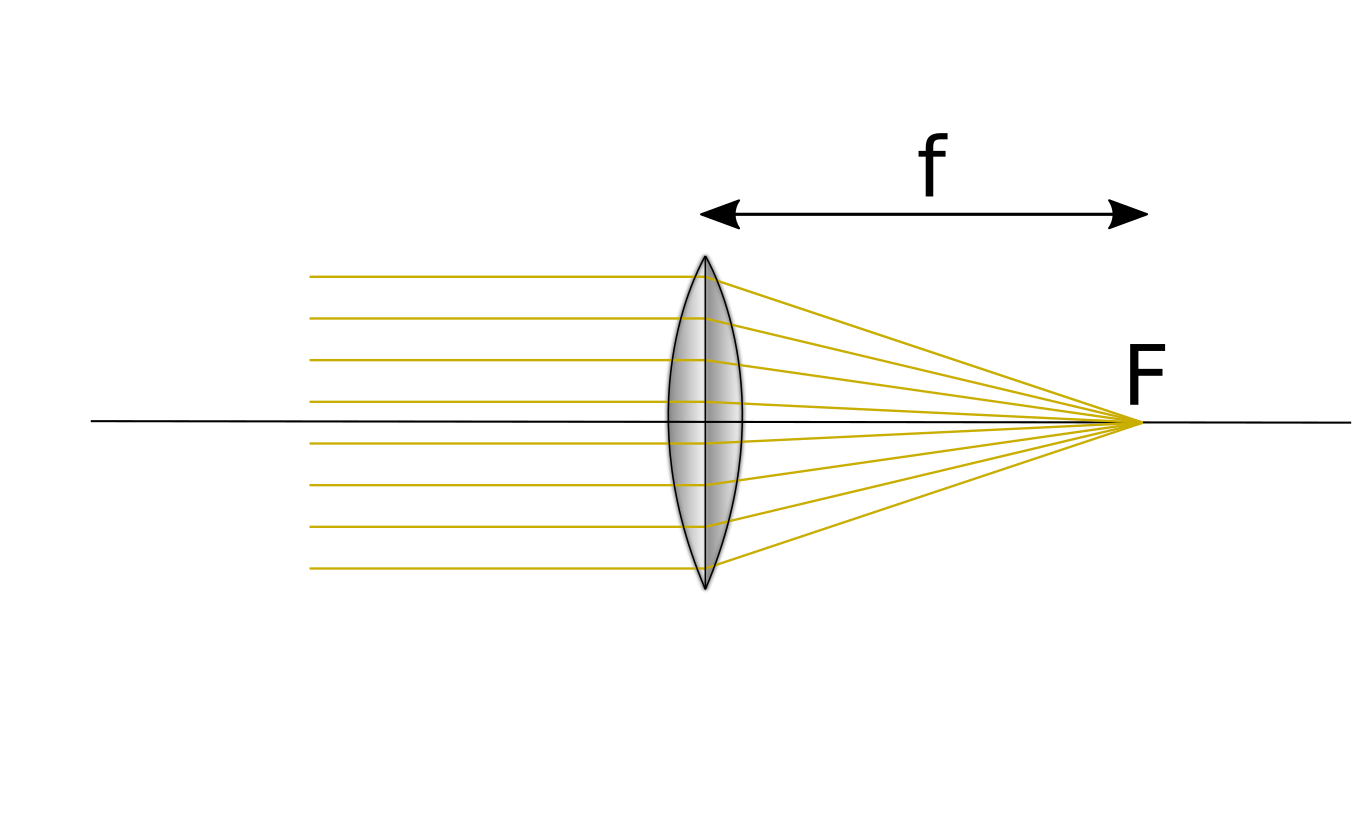
\includegraphics[scale=0.8]{Geometrische_Optik/Protokoll/fig/Versuch1.1.png}
    \caption{Einfach Bestimmung der Brennweite einer Linse}
    \label{fig:Versuch1.1}
\end{figure}

In diesem Versuchsteil soll die Brennweite einer Linse nur mit Hilfe eines Maßstabs und eines Schirms kontrolliert werden. Dazu werden sowohl Linse als auch Schirm auf einer optischen Bank montiert (Abb. \ref{fig:Versuch1.1}). Um den Fehler bei dieser Messung zu minimieren wird der Abstand zwischen Lichtquelle und Linse groß gewählt bzw. gegebenenfalls ein Kondensor nach der Lichtquelle zwischengeschaltet. Für die Messung wird nun die Linse solange verschoben, bis ein möglichst kleiner Lichtpunkt auf dem Schirm entsteht. Der Abstand zwischen Schirm und der Linse ist somit die Brennweite. Für den Versuch wird eine Linse mit einer angegebenen Brennweite von $F = 15 cm$ gewählt, dabei wird der Schirm auf der 195cm-Marke der optischen Bank fixiert. Es ergeben sich die Werte in der Tabelle \ref{tab:Daten1}. Somit ergibt sich ein Mittelwert von $16.5600$ mit einer Standardabweichung von $0.066cm$, also: $16.5600cm \pm 0.066cm$. Dies entspricht einer Abweichung von ca. $9 \% $ zum angegebenen Wert. Diese Abweichung liegt in der Ungenauigkeit der Messmethode begründet. Faktoren, die die Genauigkeit der Messung beeinflussen sind etwa, dass die Messung nicht mit monochromatischem Licht durchgeführt wurde, denn die Brechzahl hängt von der Wellenlänge des Lichts ab. Allerdings wurden zehn dicht aneinander liegende Werte ermittelt, was auch auf eine nicht korrekte Angabe der Brennweite auf der Linse hindeuten könnte. Systematische Fehler könnten aber auch die Ursache für diese große Abweichung sein, zum Beispiel, dass die Ablesemarken für die Messungen nicht genau unter der Linse, beziehungsweise unter dem Schirm liegen oder, dass die "Lichtstrahlen" nicht parallel genug für eine genaue Messung sind und somit eine größere Brennweite herauskommt, als die Linse eigentlich hat.
 
\begin{table}[h!]
    \centering
    \begin{tabular}{|c|c|}
    	\hline
    	Messung Nr. & Pos. Linse (cm) \\
    	\hline
    	1 & 178.5 \\
    	\hline
    	2 & 178.4 \\
    	\hline
    	3 & 178.4 \\
    	\hline
    	4 & 178.4 \\
    	\hline
    	5 & 178.5 \\
    	\hline
    	6 & 178.4 \\
    	\hline
    	7 & 178.5 \\
    	\hline
    	8 & 178.3 \\
    	\hline
    	9 & 178.5 \\
    	\hline
    	10 & 178.5 \\
    	\hline
    
    \end{tabular}
    \caption{Daten: Einfache Bestimmung der Brennweite einer Linse}
    \label{tab:Daten1}
\end{table}

\section{Brennweitenbestimmung einer Linse mit dem Besselverfahren}

\begin{figure}[h]
    \centering
    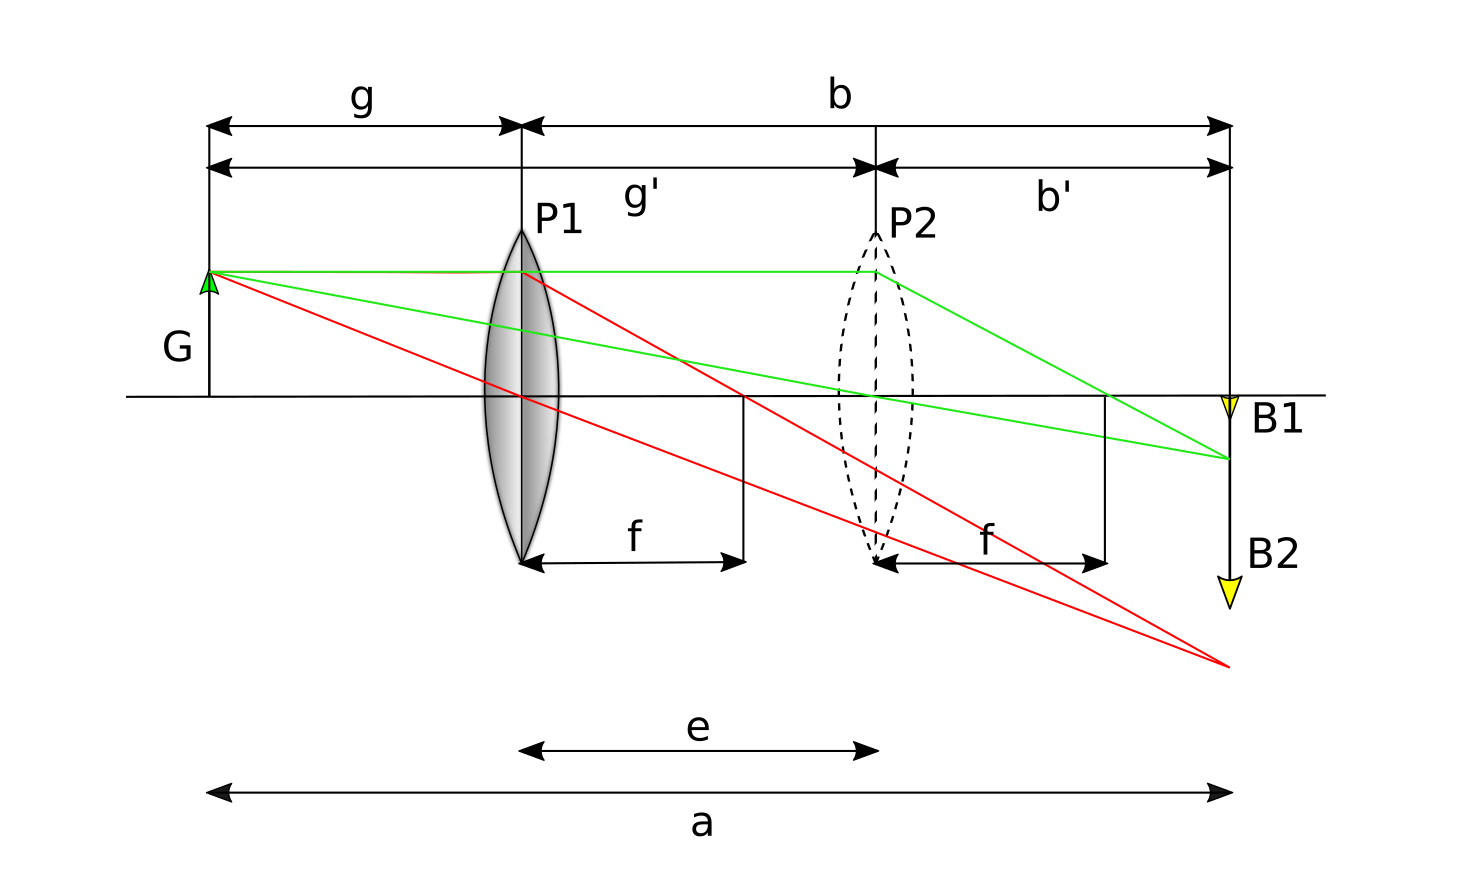
\includegraphics{Geometrische_Optik/Protokoll/fig/Besselverfahren.png}
    \caption{Besselverfahren}
    \label{fig:Besselverfahren}
\end{figure}

Zur genaueren Bestimmung der Brennweite einer dünnen Linse ist das Besselsche Verfahren gut geeignet. Dazu werden Bild (in unserem Fall ein Dia), Schirm und Linse wie in Abb. (\ref{fig:Besselverfahren}) gezeigt angeordnet. Hierbei macht man sich zu Nutze, dass es bei einem festen Abstand zwischen Bild und Schirm zwei mögliche Linsenstellungen gibt, bei denen ein scharfes Bild auf den Schirm geworfen wird. Dies soll im folgenden durch eine Herleitung gezeigt werden.
Mit einsetzen der Relationen in Gleichung \ref{Relation} in die Linsengleichung \ref{Linsengleichung}, die leicht geometrisch einzusehen ist, erhält man Gleichung \ref{Gleichung}. Diese wird für $g$ gelöst, wobei die Differenz von $g$ und $g'$ als e definiert wird (\ref{Defe}). Nach einer weiteren trivialen Umformung erhält man die Gleichung \ref{Gleichungf} für $f$.\\

\begin{equation} \label{Linsengleichung}
    \frac{1}{f} = \frac{1}{b} + \frac{1}{g}
\end{equation}

\begin{align} \label{Relation}
    b &= a - g   \\
    \nonumber b &= \frac{a-e}{2} 
\end{align}

\begin{equation} \label{Gleichung}
    \frac{1}{f} = \frac{a}{ag-g^2}
\end{equation}

\begin{equation} \label{Defe}
    e = \Delta g = \sqrt{a^2-4af}
\end{equation}

\begin{equation} \label{Gleichungf}
    f = \frac{a^2-e^2}{4a}
\end{equation}

Aus Gleichung \ref{Defe} ist sofort ersichtlich, dass für eine reelles Ergebnis $a^2 \geq 4af$ gelten muss. Außerdem ist aus selbiger auch ersichtlich, dass es nicht vorteilhaft ist $\frac{e}{f}$ zu groß zu wählen, da im Grenzfall $e = a$ gilt und somit die Linse im Bild bzw. Schirm stehen müsste. \\
Abgesehen von der eigentlichen Brennweitenbestimmung werden in diesem Versuchsteil auch zwei Linsenfehler genauer betrachtet:\\
Die chromatische und die sphärische Abberation. Dazu werden bei der Brennweitenmessung für die chromatische Rot- und Blaufilter und für die sphärische Abberation Ring- und Lochblende verwendet.\\
Bei der chromatischen Abberation handelt es sich um die Eigenschaft von Linsen, aufgrund von Dispersion, also der Abhängigkeit der Brechzahl von der Wellenlänge, beispielsweise blaues Licht stärker zu brechen als rotes. Man verwendet hier Farbfilter um die Brennweite von blauem und rotem Licht unabhängig zu messen und somit die chromatische Abberation zu bestimmen (\ref{fig:Chromatische Abberation}).\\
Die sphärische Abberation ist ein Linsenfehler bei dem, im Normalfall, achsennahes Licht weniger stark gebrochen wird, als achsenfernes Licht. Die Brennweite für achsenahes Licht fällt also größer aus, als die Brennweite für achsenfernes Licht. Um diesen Linsenfehler qualitativ zu beschreiben werden in zwei Messungen jeweils eine Loch- bzw. Ringblende vor der Linse fixiert und damit für achsennahes und achsenfernes Licht separat die Brennweiten gemessen (\ref{fig:Sphärische Abberation}).\\
Es wird jeweils einmal für den Blaufilter, Rotfilter, Ringblende und Lochblende ein Set mit je 4 unabhängigen Messungen für die beiden möglichen Kofirugationen (kleineres und größeres scharfes Bild) erstellt, wobei die ersten zwei Messungen von Person 1 und die anderen zwei von Person 2 durchgeführt wurden um personenabhängige Fehler einzugrenzen. Von jedem der insgesamt 8 Sets wird der Mittelwert ermittelt und daraus die entsprechende Brennweite errechnet.

\begin{figure}[h!]
    \centering
    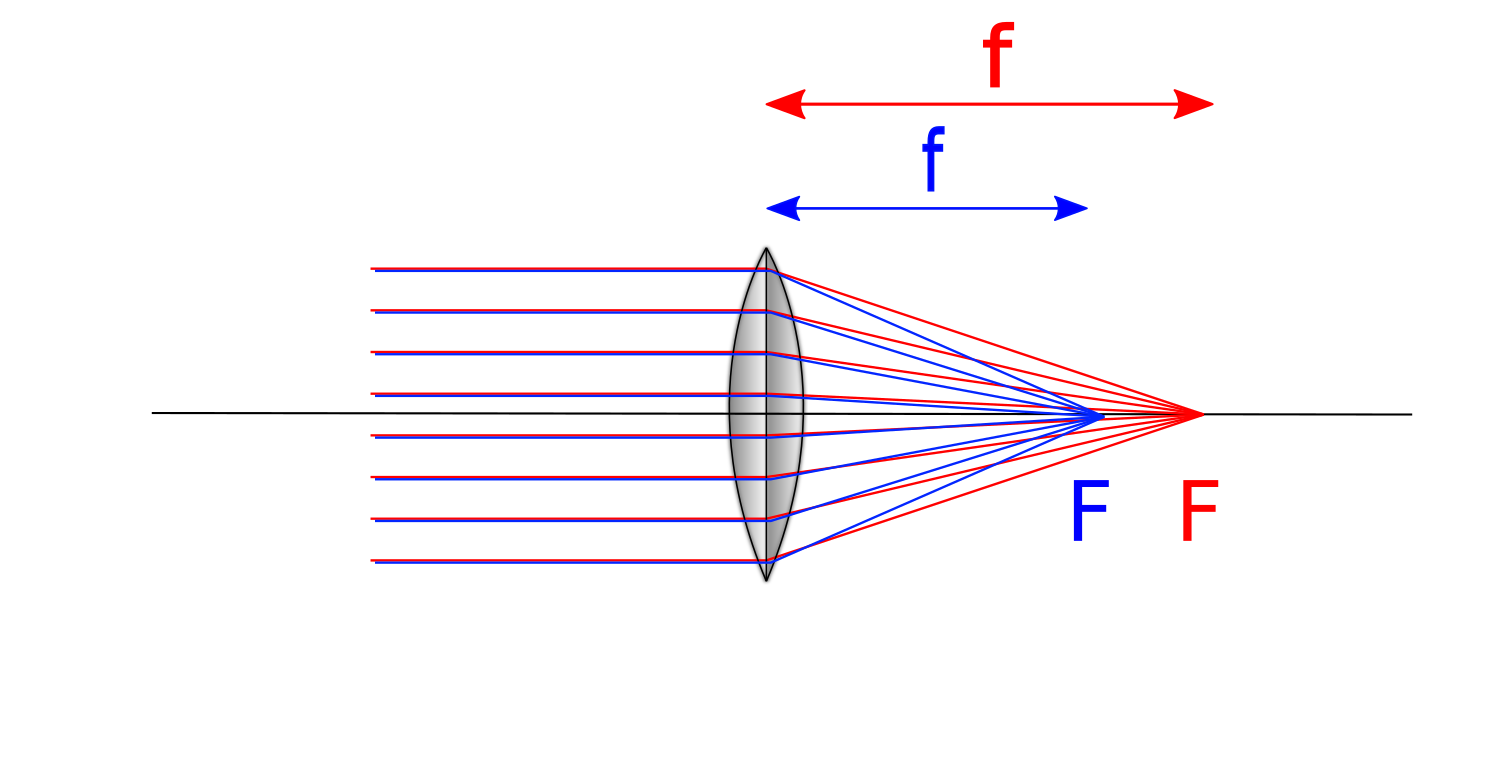
\includegraphics[scale=0.8]{Geometrische_Optik/Protokoll/fig/Chromatische Abberation.png}
    \caption{Chromatische Abberation}
    \label{fig:Chromatische Abberation}
\end{figure}

\begin{figure}[h!]
    \centering
    \includegraphics[scale=0.8]{Geometrische_Optik/Protokoll/fig/Sphärische Abberation.png}
    \caption{Sphärische Abberation}
    \label{fig:Sphärische Abberation}
\end{figure}

\clearpage

\subsection{Fehlerrechnung zur Brennweitenbestimmung einer Linse mit dem Besselverfahren}
Der Fehler wird aus der Ungenauigkeit des Maßstabs, die als $0.5mm$ (halbe Skala) abgeschätzt wird und aus dem ungenauen Winkel der Halterungen, abgeschätzt, wobei für letzteres ein Winkel von einem halben Grad als sinnvolle Ungenauigkeit erachtet wird und die Linsen ungefähr auf einer Höhe von $150mm$ angebracht sind. Somit ergibt sich insgesamt eine Ungenauigkeit von $0.5mm + \sin{0.5} = 1.5mm$
Für den Fehler auf die Mittelwerte gilt allgemein: $\sigma = \sigma_x / \sqrt{N}$ wobei $\sigma$ der resultierende Fehler ist, $\sigma_x$ der Fehler auf die Einzelmessung und $N$ die Anzahl der Messungen, wir erhalten folglich einen Fehler von $0.75mm$.
Mit der gaußschen Fehlerfortpflanzung erhalten wir für den Abstand zwischen den möglichen Linsenstellungen $e$ und für die Brennweite $f$:

\begin{equation}
    \sigma_f = \sqrt{\sum_{j=1}^m(\frac{\partial f}{\partial x_j})^2 \cdot \sigma_{x_j}^2} 
    =\sqrt{(\frac{\partial f}{\partial a})^2 \cdot \sigma_{a}^2 + (\frac{\partial f}{\partial a})^2 \cdot \sigma_{a}^2} 
    =\sqrt{\frac{1}{4}(1+(\frac{e}{a})^2)^2 \cdot \sigma_a + (\frac{-e}{2a})^2 \cdot \sigma_e}
\end{equation}

\begin{equation}
    \sigma_e
    =\sqrt{(\frac{\partial e}{\partial g_1})^2 \cdot \sigma_{g_1}^2 + (\frac{\partial e}{\partial g_2})^2 \cdot \sigma_{g_2}^2} 
    =\sqrt{(\sigma_{g_1})^2 + (\sigma_{g_2})^2}
\end{equation}

Damit ergibt sich:\\

\begin{table}[h!]
    \centering
\begin{tabular}{|c|c|c|c|c|}
	\hline
	& Blaufilter & Rotfilter & Lochblende & Ringblende \\
	\hline
	Mittelwert von e (cm) & 18.42 & 17.54 & 17.52 & 17.65 \\
	\hline
	Fehler auf e (cm) & 0.106 & 0.106 & 0.106 & 0.106 \\
	\hline
	Mittelwert von f (cm) & 13.58 & 13.71 & 13.72 & 13.70 \\
	\hline
	Fehler auf f (cm) & 0.043 & 0.043 & 0.043 & 0.043 \\
	\hline
\end{tabular}
    \caption{Mittelwerte und Fehler für e und f}
    \label{tab:Mittelwerte}
\end{table}

An den Werten der Tabelle (\ref{tab:Mittelwerte}) ist klar ersichtlich, dass es eine große Abweichung zum auf der Linse angegebenen Wert gibt, der auch nicht mehr innerhalb des Fehlers liegt. Dies kann an verschiedenen Faktoren liegen: \\

\begin{itemize}
\item die Beschriftung der Linse ist nicht korrekt
\item es wurde bei einer anderen Wellenlänge gemesse
\item es wurde deutlich näher an der Achse gemessen
\item es handelt sich um personenabhängige Fehler
\end{itemize}

Der letzte Punkt kann nahezu ausgeschlossen werden, da alle Werte nah beieinander liegen.
Auch eine große Streuung ist nicht feststellbar.\\
Eine andere Erklärung wäre, dass sich das Bild nicht zu 100\% scharf stellen lässt, da bei dieser Linse entweder der innere Bereich des Bilds scharf gestellt werden konnte oder der äußere. Außerdem lässt sich deutlich die Abweichung von dem Ergebnis der einfachen Brennweitenbestimmung erkennen, was wahrscheinlich der genaueren Messmethode zu verdanken ist.\\
Abgesehen davon kann man an den Mittelwerten, in Verbindung mit den Fehlern für die Brennweiten der einzelnen Konfigurationen, relativ deutlich die chromatische Abberation der Linse erkennen. Dahingegen lässt sich die spärische Abberation nur kaum bis gar nicht erkennen, vor allem mit dem errechneten Fehler. Daher lässt sich auf eine geringe spärische Abberation schließen.


\section{Brennweitenbestimmung eines Zweilinsensystems mit dem Abbéschen Verfahren}

\begin{figure}[h!]
    \centering
    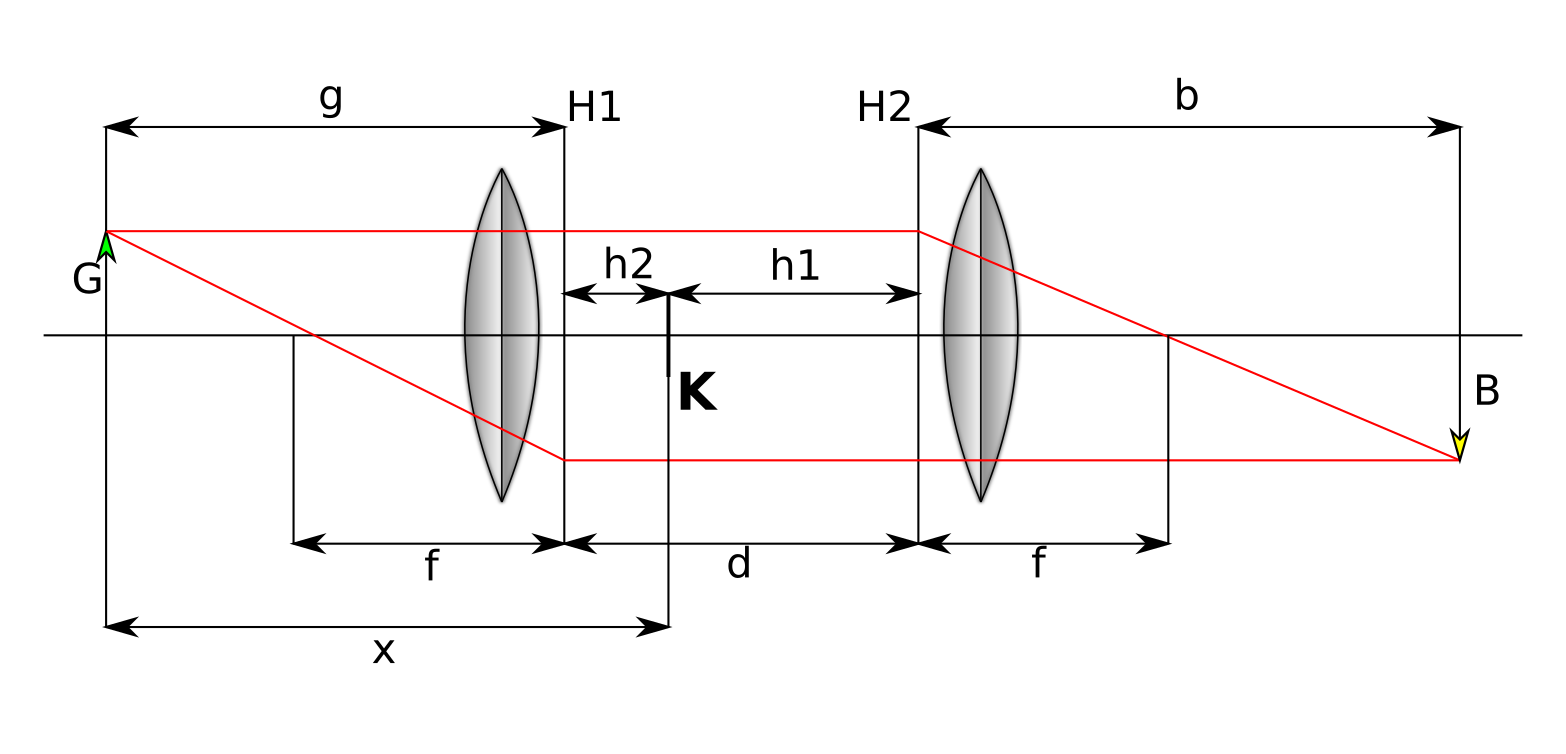
\includegraphics[scale=0.8]{Geometrische_Optik/Protokoll/fig/Abbeverfahren.png}
    \caption{Abbeverfahren}
    \label{fig:Abbeverfahren}
\end{figure}

Während mit dem Besselverfahren die Brennweite einer einzelnen Linse bestimmt wird, lassen sich mit dem Abbeverfahren die Brennweiten und Hauptebenen eines Linsensystems bestimmen.
Für diesen Versuch wurde ein Linsensystem aus zwei Linsen in einem Rohr verwendet, die sich innerhalb des Rohres unhabhänging voneinander verschieben lassen.
Das Rohr wird an einem festen Punkt K auf der optischen Bank befestigt.

Für das Linsensystem ergibt sich mit dem Abbildungsmßaßstab $\gamma = B/G = b/g$

\begin{equation} \label{Linsensystem}
    g = f(1 + \frac{1}{y}),/ b = f(1+y)
\end{equation}

Wobei g und b jeweils die Abstände zwischen Gegenstand bzw. Bild und dessen zugeordneten Hauptebene sind und B und G die Bild- und Gegenstandsgröße repräsentieren.
Da die Lage der Hauptebenen bei einem Linsensystem nicht ohne weiteres bekannt ist, können g und b nicht direkt durch Messung bestimmt werden und müssen in der Gleichung
durch messbare Werte ersetzt werden.
Dies geschieht wie folgt:

Man ordnet zunächst dem Gegenstand die Hauptebene $h_1$ der vorderen Linse zu, sodass sich für den Abstand zwischen Gegenstand und K ergibt

\begin{equation} \label{x1}
    x = g + h_1
\end{equation}

Nun setzt man hier \ref{Linsensystem} ein:

\begin{equation} \label{x2}
    x = f(1 + \frac{1}{y}) + h
\end{equation}

und eleminiert durch Umstellen und Einsetzen $h_1$, um eine Gleichung für $f_1$ zu erhalten.

\begin{equation} \label{1}
    h_1 = x_2 - f(1 + \frac{1}{y_2})
\end{equation}

\begin{equation} \label{3}
    f_1 = \frac{x_1 - h}{(1 + \frac{1}{y_1})}
\end{equation}

\begin{equation} \label{4}
    f_1 = \frac{x_2 - x_1}{(\frac{1}{y_2} + \frac{1}{y_1})}
\end{equation}

Wenn man nun mit zwei Messwertpaaren $(x_1, y_1), (x_2, y_2)$ f errechnet, kann man dieses in \ref{1} verwenden um $h_1$ zu erhalten.

Um die 2. Hauptebene $H_2$ zu bestimmen, wird das Rohr auf dem Punkt um 180° gedreht und analog vorgegangen:

\begin{equation} \label{4}
    f_2 = \frac{x_2' - x_1'}{(\frac{1}{y_2'} + \frac{1}{y_1'})}
\end{equation}

Entsprechend der Mathematik wurde der Abstand zwischen Gegenstand und Linsensystem durch versetzen des Gegenstandes verändert und das Bild danach durch re-positionieren des Schirms scharfgestellt.
Um die resultierende Größenänderung des Bildes sinnvoll messen zu können, wurde als Gegenstand ein Dia mit einem 1cm Strich verwendet, und auf dem Schirm Millimeterpapier angebracht.

Im Versuch wurden zwei Messreihen für jeweils unterschiedliche Linsenabstände aufgenommen und Abwechselnd für die Ausgangs- und die um 180° gedrehte Position des Systems gemessen.

\begin{table}[h!]
    \begin{center}
        \caption{Daten: Abbe-Verfahren für Zweilinsensystem bei 11.5cm Linsenabstand$S_1$}
        \begin{tabular}{ccc}
            \hline
            Rotation   &  Vergrößerung  $X$ in $\SI{}{cm}$    & Abstand$V$ \\
            \hline
            \multirow{6}{*}{\SI{0}{\degree}}    & $\SI{1.8}{}$ & $\SI{15}{}$ \\
                                                & $\SI{0.9}{}$ & $\SI{20}{}$ \\
                                                & $\SI{2.1}{}$ & $\SI{14}{}$ \\
                                                & $\SI{1.5}{}$ & $\SI{16}{}$ \\
                                                & $\SI{1.3}{}$ & $\SI{17}{}$ \\
                                                & $\SI{2.3}{}$ & $\SI{13.5}{}$ \\
            \hline
            \multirow{6}{*}{\SI{180}{\degree}}  & $\SI{1.2}{}$ & $\SI{15}{}$ \\
                                                & $\SI{0.7}{}$ & $\SI{20}{}$ \\
                                                & $\SI{1.3}{}$ & $\SI{14}{}$ \\
                                                & $\SI{1.1}{}$ & $\SI{16}{}$ \\
                                                & $\SI{0.9}{}$ & $\SI{17}{}$ \\
                                                & $\SI{1.4}{}$ & $\SI{13.5}{}$ \\
            \hline
            \label{tab:Abbe1}
        \end{tabular}
    \end{center}
\end{table}

\begin{table}[h!]
    \begin{center}
        \caption{Daten: Abbe-Verfahren für Zweilinsensystem bei 9.5cm Linsenabstand$S_1$}
        \begin{tabular}{ccc}
            \hline
            Rotation   &  Vergrößerung  $X$ in $\SI{}{cm}$    & Abstand$V$ \\
            \hline
            \multirow{6}{*}{\SI{0}{\degree}}    & $\SI{1.7}{}$ & $\SI{85}{}$ \\
                                                & $\SI{0.7}{}$ & $\SI{80}{}$ \\
                                                & $\SI{2.0}{}$ & $\SI{86}{}$ \\
                                                & $\SI{1.4}{}$ & $\SI{84}{}$ \\
                                                & $\SI{1.2}{}$ & $\SI{83}{}$ \\
                                                & $\SI{2.3}{}$ & $\SI{86.5}{}$ \\
            \hline
            \multirow{6}{*}{\SI{180}{\degree}}  & $\SI{1.1}{}$ & $\SI{85}{}$ \\
                                                & $\SI{0.6}{}$ & $\SI{80}{}$ \\
                                                & $\SI{1.3}{}$ & $\SI{86}{}$ \\
                                                & $\SI{1.0}{}$ & $\SI{84}{}$ \\
                                                & $\SI{0.9}{}$ & $\SI{83}{}$ \\
                                                & $\SI{1.3}{}$ & $\SI{86.5}{}$ \\
            \hline
            \label{tab:Abbe2}
        \end{tabular}
    \end{center}
\end{table}

\clearpage

\subsection{Fehlerrechnung zur Brennweitenbestimmung eines Zweilinsensystems mit dem Abbéschen Verfahren}

Zur Berechnung der Werte $f_1,\ h_1,\ f_2\ und\ h_2$ werden die Messwerte der beiden Messreihen unter Regression geplottet.
Zur Approximation wurde die lineare Funktion $f(x) = m \cdot x + c$ verwendet, wobei 

[Anmerkung von Linn:
Ich bin bei der Auswertung der Messreihen in ein technisches Problem mit Python gerannt, dass ich nicht mehr rechtzeitig vor der Abgabe lösen konnte.
Ich werde das Problem beheben und den fehlende Teil bei der 2. Abgabe hinzufügen.]
    
    \chapter{Aufbau optischer Instrumente (Versuchsteil 2)}
    \section{Bau zwei verschiedener Fernrohre}
\subsection{Keplersches Fernrohr}

In diesem Versuchsteil geht es darum ein Keplersches Fernrohr zu bauen und dabei mindestens eine Vergrößerung von 6 zu erreichen. Dazu werden zwei Linsen mit verschiedenen Brennweiten so auf einer optische Bank befestigt, dass sie einen Abstand von $$ d = f_1 + f_2 $$ haben. Um die gewünschte Vergrößerung zu erreichen wählt man die Linsen so, dass die Formel für die Vergrößerung mindestens 6 ergibt. $$  \gamma = \frac{f_1}{f_2} \geqslant 6$$Gewählt wird eine für die erste Linse eine Brennweite von $500mm$ und für die zweite eine Brennweite von $70mm$, was eingesetzt in die Formel für die Vergrößerung eine theoretische Vergrößerung von $\thickapprox 7,14 $ ergibt. Der Abstand zwischen den Linsen muss demnach $d = 700mm + 50mm = 57cm$ betragen.
Um die experimentelle Vergrößerung zu ermitteln wird der Okulardurchmesser gemessen und der durch das Fernrohr sichtbare Bereich gemessen, dies entspricht der Bild- und Gegenstandsgröße, somit kann mit der Formel $$ \gamma = \frac{B}{G} $$ die Vergrößerung berechnet werden. Mit den Werten aus der Tabelle \ref{tab:Tabellekeppler} ergibt sich eine Vergrößerung von $10$. Was einer relativ großen Abweichung vom theoretischen Wert entspricht. Was wahrscheinlich auf die ungenaue Methode die Vergrößerung zu messen zurückzuführen ist.

\begin{table}[h]
    \centering
    \begin{tabular}{|c|c|}
	\hline
	f1\ & 500mm \\
	\hline
	f2\ & 70mm \\
	\hline
	Theoretische Vergrößerung  & 7,14 \\
	\hline
	Okulardurchmesser & 31mm \\
	\hline
	Sichtbarer Bereich & 310mm \\
	\hline
	Exp. gemessene Vergrößerung & 10 \\
	\hline
    \end{tabular}
    \caption{Messwerte Keplersches Fernrohr}
    \label{tab:Tabellekeppler}
\end{table}

\begin{figure}
    \centering
    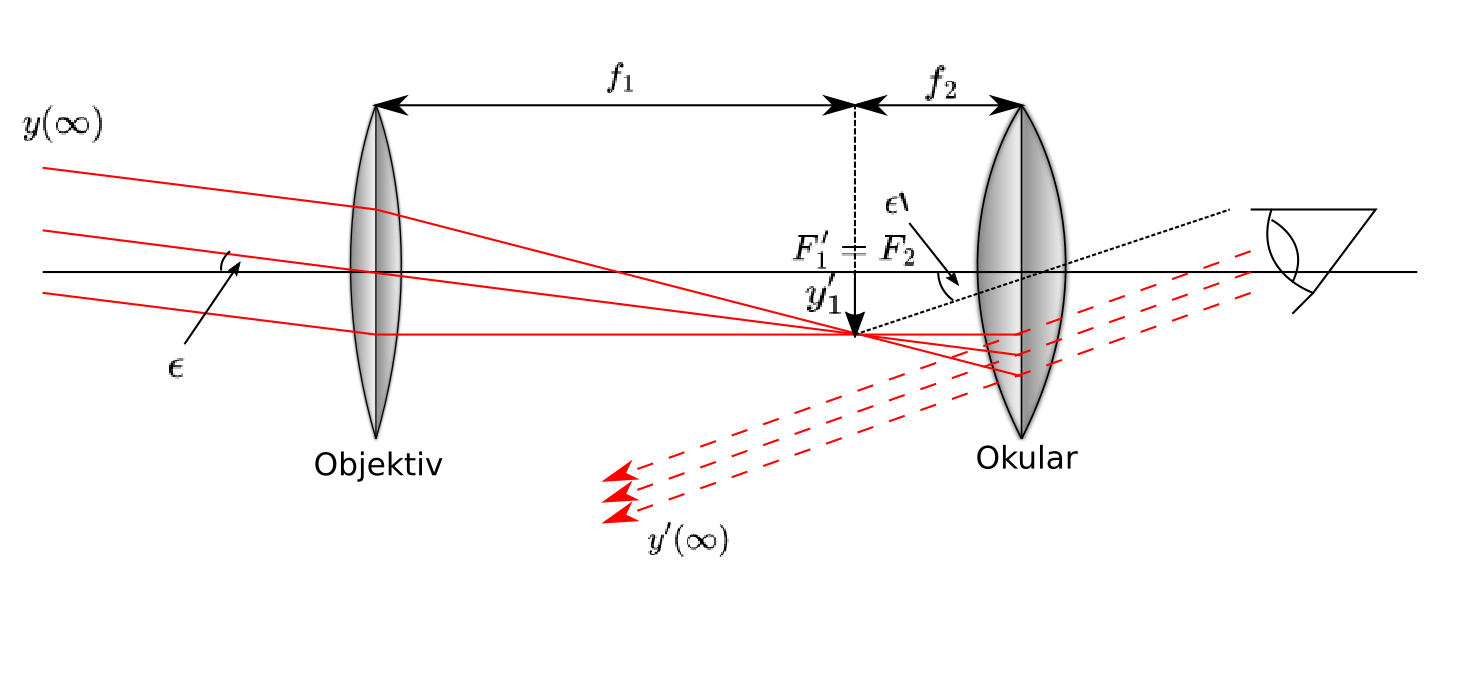
\includegraphics[scale=0.8]{Geometrische_Optik/Protokoll/fig/Keplerfernrohr.png}
    \caption{Keplerfernrohr}
    \label{fig:Keplerfernrohr}
\end{figure}

\subsection{Galileisches Fernrohr}
Die Besonderheit des Galileischen Fernrohrs gegenüber dem Keplerschen, ist, dass es sich eine Zerstreuungslinse zur Nutze macht, dadurch steht das Bild nicht mehr auf dem Kopf, außerdem lässt sich mit dieser Bauart eine geringe Baulänge erreichen bei gleicher Vergrößerung. Die Vergrößerung lässt sich ähnlich wie beim Galileischen Fernrohr berechnen: $$ \gamma = \frac{f_1}{|f_2|} $$ Wobei die Baulänge und somit der Abstand der Linsen $$ d = f_1' - |f_2| $$ beträgt. Für diesen Versuch werden Linsen mit den Brennweiten $f_1 = 500$ und $f_2 = -100$ gewählt. Nach obiger Formel müssen die Linsen einen Abstand von $400mm$ haben. Errechnet werden wieder theoretische Vergrößerung und experimentell bestimmte Vergrößerung, es ergeben sich die in Tabelle \ref{tab:Tabellegalileo} aufgeführten Werte.

\begin{table}[h]
    \centering
\begin{tabular}{|c|c|}
	\hline
	f1 & 500mm \\
	\hline
	f2 & -10mm \\
	\hline
	Theoretische Vergrößerung & 5 \\
	\hline
	Okulardurchmesser & 8mm \\
	\hline
	Sichtbarer Bereich & 341mm \\
	\hline
	Exp. gemessene Vergrößerung & 4.26 \\
	\hline
    \end{tabular}
    \caption{Messwerte Gelileisches Fernrohr}
    \label{tab:Tabellegalileo}
\end{table}

\begin{figure}
    \centering
    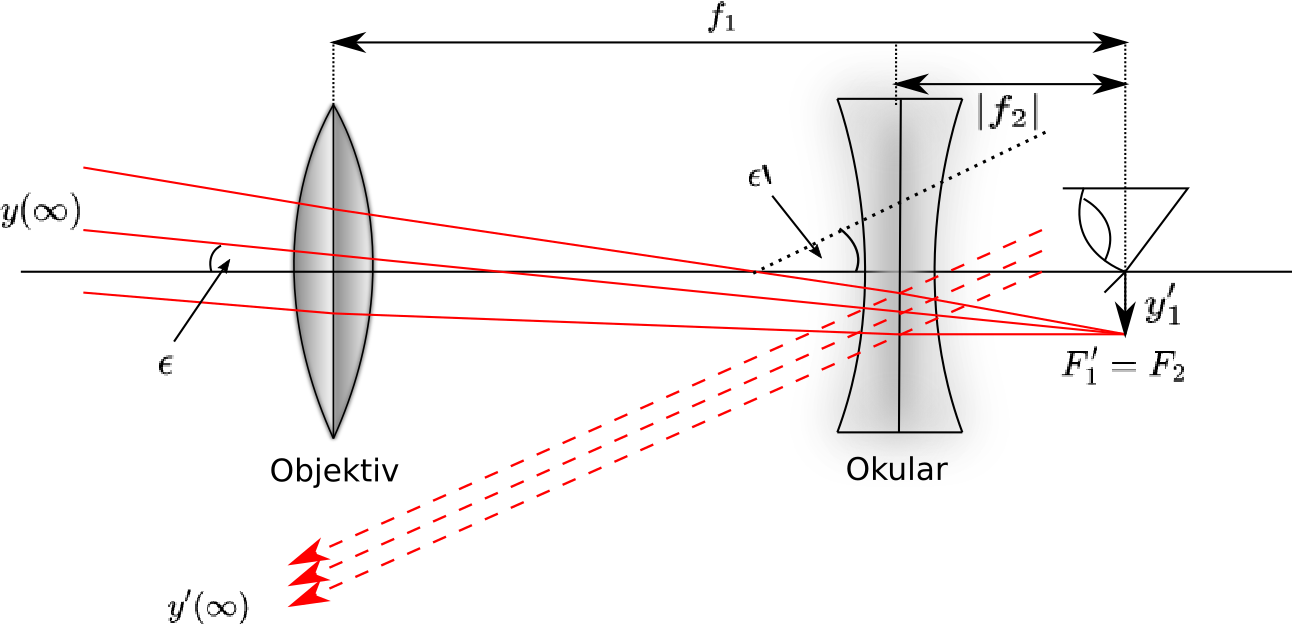
\includegraphics[scale=0.8]{Geometrische_Optik/Protokoll/fig/Galileofernrohr.png}
    \caption{Galileofernrohr}
    \label{fig:Galileofernrohr}
\end{figure}

\section{Bau eines Projektionsapparats}

Es soll ein Projektionsapparat gebaut werden mit dem Dias auf eine $1.5m$ mit ungefähr 10-facher Vergrößerung abgebildet werden können. Dafür wird eine Linse zusammen mit einem Diahalter und einem Schirm, wie in Abbildung \ref{fig:Diaprojektor} aufgebaut. Dabei werden die Abstände so gewählt, dass sich die Gegenstandsweite und die Bildweite, wie in Tabelle \ref{tab:Diaprojektor} aufgeführt, ergeben. Die theoretische Vergrößerung lässt sich nun mit der Formel: $$ \gamma = \frac{b}{g} $$ berechnen. Die experimentelle Vergrößerung wird hingegen mit einem Dia mit einem ein Zentimeter langen Strich gemessen, indem die Größe diese Strichs auf dem Schirm gemessen wird. Dabei ergeben sich für die theoretische und experimentell bestimmte Vergrößerung die Werte die in der Tabelle \ref{tab:Diaprojektor} aufgeführt sind.

\begin{table}[]
    \centering
    \begin{tabular}{|c|c|}
	\hline
	Gegenstandsweite & 10,8 \\
	\hline
	Bildweite & 118,2 \\
	\hline
	Vergrößerung (theoretisch) & 10,94 \\
	\hline
	Vergrößerung (experimentell) & 10.5 \\
	\hline
\end{tabular}
    \caption{Diaprojektor}
    \label{tab:Diaprojektor}
\end{table}


\begin{figure}
    \centering
    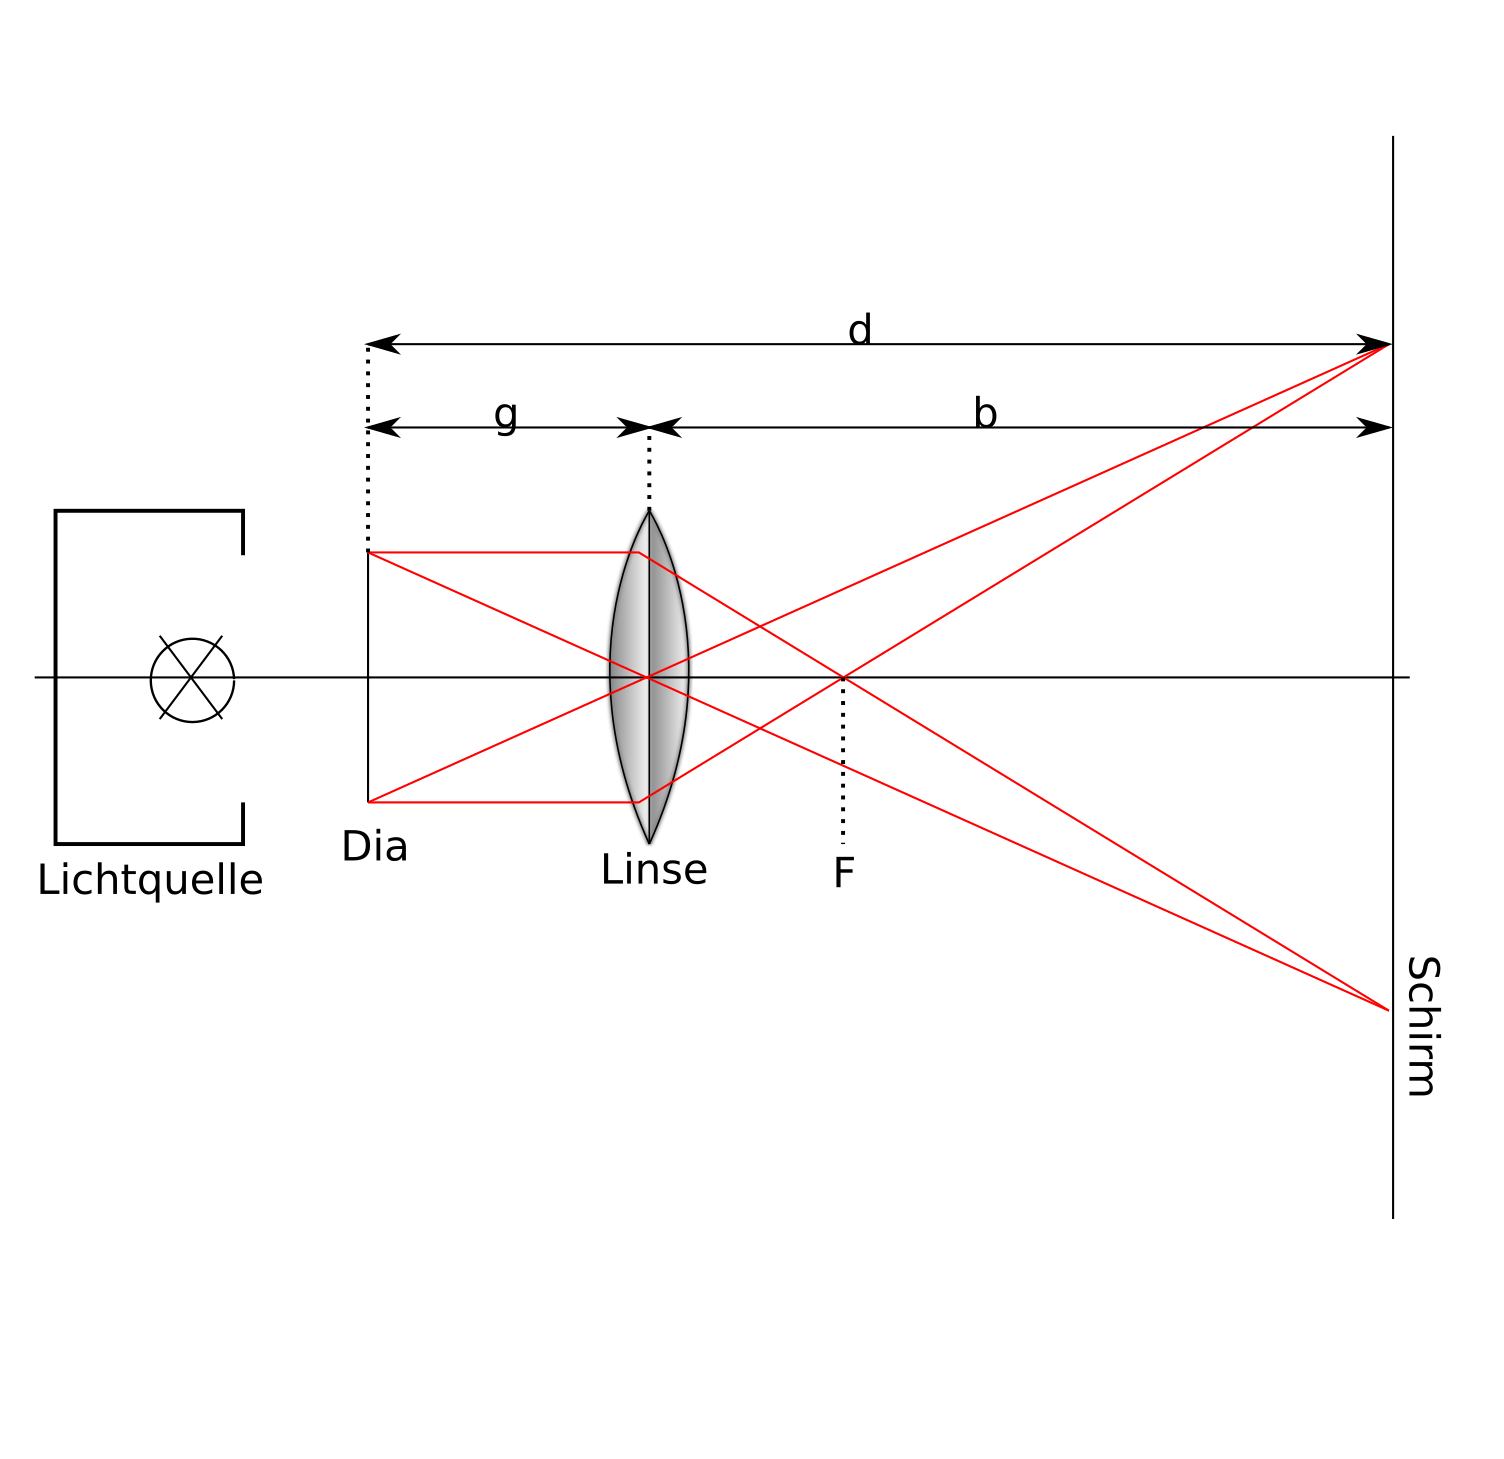
\includegraphics[scale=0.8]{Geometrische_Optik/Protokoll/fig/Diaprojektor.png}
    \caption{Diaprojektor}
    \label{fig:Diaprojektor}
\end{figure}

\section{Bau eines Mikroskops}
Es soll ein Mikroskop mit mindestens zwanzigfacher Vergrößerung gebaut werden, dazu werden zwei Linsen nach der Abbildung \ref{fig:Mikroskop} aufgebaut, die Brennweiten für die beiden Linsen werden nach der Formel: $$ \gamma = \frac{b \cdot s_0}{g \cdot f_2 } \approx \frac{(d - f_2) \cdot s_0}{f_1 \cdot d_2}$$ bestimmt, wobei $s_0 = 250mm$. Es werden die Brennweiten $f_1 = 500mm$ und $f_2 = 70mm$ gewählt, was eingesetzt in die Formel eine Vergrößerung von 4,14 ergibt. Was nicht der gewollten Vergrößerung entspricht. Allerdings lässt sich auch so schon die Funktionsweise des Mikroskops erkennen, man müsste lediglich die Linsen anders wählen um eine größere Vergrößerung zu erreichen.

\begin{figure}
    \centering
    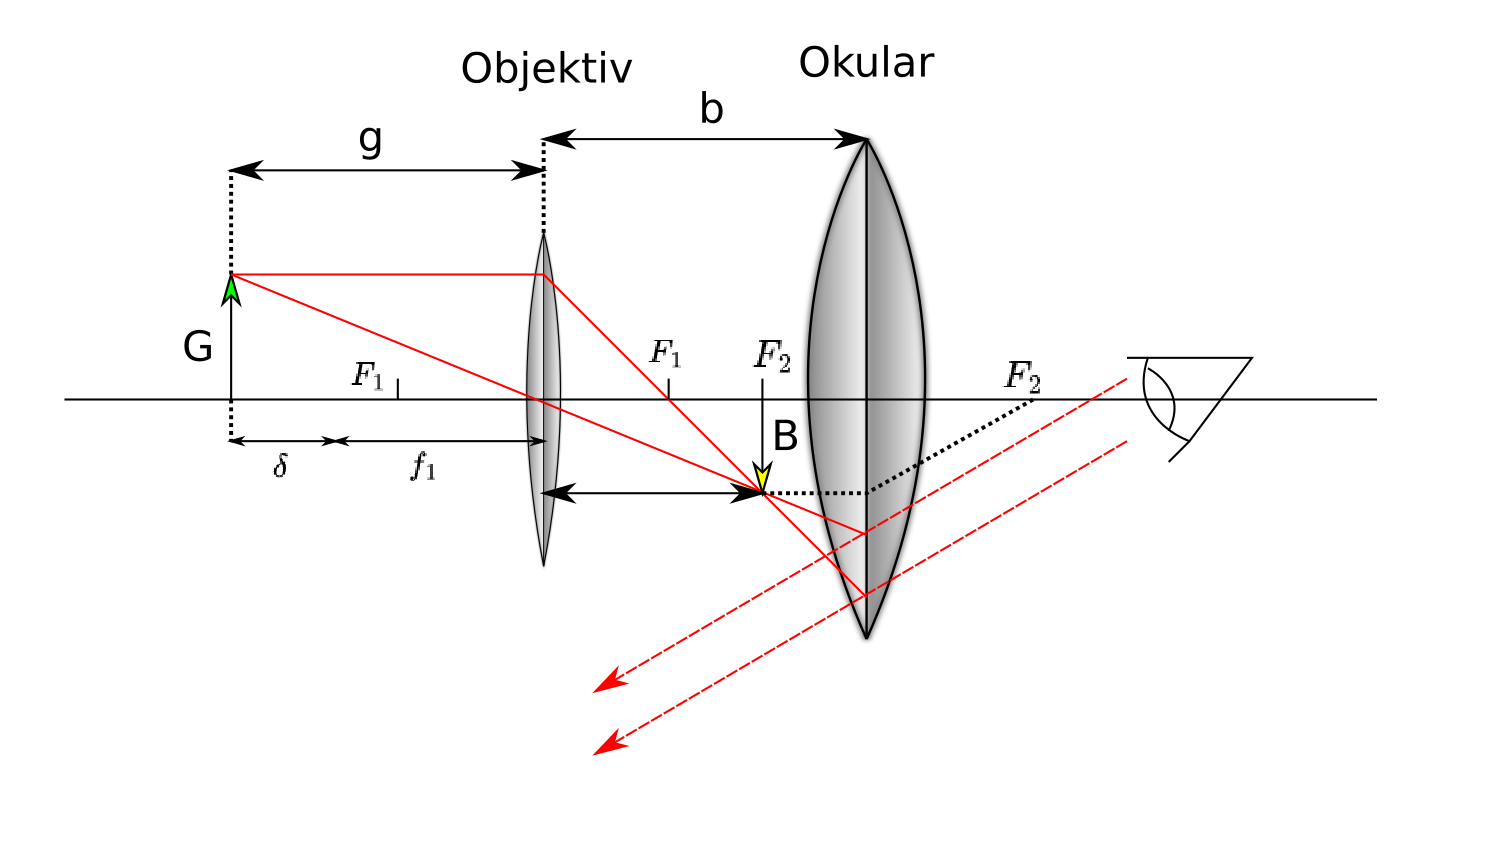
\includegraphics[scale=0.8]{Geometrische_Optik/Protokoll/fig/Mikroskop.png}
    \caption{Mikroskop}
    \label{fig:Mikroskop}
\end{figure}

    
    %\chapter{Auswertung}
    %Ganz tolle Auswertung des Versuchs. \cite{Dem10} %\cleardoublepage

    % appendix for more or less interesting calculations
    % \Appendix
    %\chapter*{\appendixname} \addcontentsline{toc}{chapter}{\appendixname}
    % to make the appendix appear in ToC without number. \appendixname = 
    % Appendix or Anhang (depending on chosen language)
    %\section{Erster Abschnitt des Anhangs}
Dies ist der erste ganz tolle Abschnitt des Anhangs. %\cleardoublepage



    % Bibliography
    \TheBibliography

    % BIBTEX
    % use if you want citations to appear even if they are not referenced to: 
    % \nocite{*} or maybe \nocite{Kon64,And59} for specific entries
    %\nocite{*}
    \bibliographystyle{babalpha}
    \bibliography{lit.bib}

    % THEBIBLIOGRAPHY
    %\begin{thebibliography}{000}
    %    \bibitem{ident}Entry into Bibliography.
    %\end{thebibliography}
\end{document}
